\section{Exascale}\label{sec:exascale}



\section{Le domaine du HPC en 2017: challenges et contraintes}


\begin{fancyquotes}
Peu importe quelle puissance attendront les processeurs, le logiciel trouvera toujours une façon d'utiliser cette puissance. Construisez un processeur 10 fois plus rapide, et la partie logiciel trouvera toujours 10 fois plus à faire (ou le fera 10 fois moins efficacement)  \cite{sutter2005software}
\end{fancyquotes}


Dans cette section nous allons tout d'abord exposer quels sont les challenges du HPC en 2017, pourquoi nous en avons besoin plus que jamais. Dans une seconde partie nous aborderons les contraintes qui empêchent les super-calculateurs de continuer à augmenter leur puissance d'années en années comme cela se faisait jusqu'à maintenant.

\subsection{Les challenges et opportunités}

La création de cette collaboration entre l'école de l'ENS et HPE n'est pas due au hasard. Cette thèse a été créée alors que le domaine du HPC connais un ralentissement sans précèdent (graphique \ref{pic_top500perf_evo}. Depuis 2012 certaines barrières ont été atteintes et les processus qui permettaient aux architectures d'évoluer à cadence constante ne sont plus viables. 




\subsubsection{Exascale}
Aujourd'hui nous rencontrons des utilisations du HPC tous les jours, que ce soit quand nous regardons la télévision ou que nous consultons le cours de la bourse. Le HPC à un réel impacte sur nos vie, les rendant plus sécurisées en prévoyant précisément des catastrophes naturelles. tous les jours de nouvelles applications sont découvertes, et certaines ne sont techniquement pas envisagées car elles nécessiteraient trop de puissances de calculs. L'objectif de tous les constructeurs présent dans le domaine du HPC est la construction du premier ordinateur capable de réaliser  $10^18$ opérations sur des nombres rationnels par secondes, l'équivalent d'un \textit{exaflop} ($10^18$ Floating Point Operations). L'industrie s'est donc lancée dans cette course effrénée à l'exaflop. En effet, le premier constructeur qui y parviendra bénéficiera d'un grand coup marketing et acquerra de nombreux clients car la majorité des clients ont des problèmes ne pouvant être réglé que par un ordinateur de cette puissance, et attendent son arrivé.

\subsubsection{De nouveaux clients}
L'arrivée de l'exaflop va entrainer l'arrivée de nouveaux clients, et il est indispensable pour des constructeurs comme HPE d'être prêt à les accompagner. Avec l'apparition des objets connectés le monde connaît une explosion des données qui sont générées et collectées. Elles sont ensuite stockées dans des data centers, qui n'ont pas les puissances suffisantes pour pouvoir les analyser. En effet les données générées par les montres, les frigos connectés ou les capteurs dans des chaînes de productions n'ont pas réelle utilité si elles ne sont pas exploité grâce à des techniques de \textit{Data Mining}. Et l'arrivée du machine learning nous ouvre à un monde extraordinaire qui n'est possible que si nous créons les architectures adéquats pour en profiter. Un autre domaine nécessitant ces quantités de calculs est celui de la recherche médicale et biologique. Aujourd'hui nous sommes capables de simuler des réactions chimiques de quelques nano secondes et sur de petit volumes. La création de supercalculateur exaflopique serait une énorme avancée pour ces clients, et les constructeurs qui n'auront pas misé sur l'exascale seront terriblement impactés. Ces nouveaux clients sont une grosse opportunité pour une entreprise comme HPE. Une analyse de marché paru en 2016 montre que le marché du High Performance Computing pèsera 36 milliards de dollars en 2020, alors qu'il en valait 28 en 2015\footnote{\url{http://www.marketsandmarkets.com/Market-Reports/Quantum-High-Performance-Computing-Market-631.html}}. Cette augmentation de 5\% par année est due à l'explosion des quantités, à la complexité des techniques pour les analyser et les visualiser et de la demande grandissante de solution HPC dans de nombreux domaines.


\subsubsection{Les nouvelles technologies}
Dans l'objectif de construire des supercalculateur toujours plus puissant nous pouvons et allons pouvoir nous appuyer sur des évolutions technologiques majeures. En effet que ce soit au niveau des mémoires avec l'arrivée des mémoire non-volatile (NVM memory), ou au niveau des réseaux avec la photonics. Il va falloir que, constructeur comme client, se tienne à jour de toutes ces évolutions technologique qui vont modifier les façon de programmer et de construire les architectures. HPE à un un projet de machine exascale nommé The Machine. Cette architecture très novatrice s'appuie sur trois piliers technologiques: les mémoires \textit{memristors} et les réseaux à base de fibre: la \textit{ photonic}. La troisième avancée et la restructuration complète de l'architecture d'un super calculateur grâce au protocole de communication Gen-Z.\\

%*****************************************************************************************************

\subsection{Les contraintes}
La loi de Moore prevoyait une augmentation exponetielle de la puissance des processeurs, mais une telle augmentation ne peut pas continuer indéfiniment car nous avons atteints certaines limites physiques. La course à l'exascale est lancée mais il existe beaucoup de contraintes qui ralentissent et compliquent ce challenge technologiques. Les contraintes sont multiples et n'influe pas autant sur les performances, mais depuis 2012 on assiste à un changement de dynamique (voir le graphique \ref{pic_top500perf_evo}). Cette partie liste donc les contraintes majeures qui impactent le domaine du calcul haute performance.


\subsubsection{Électrique}
L'électricité est une forte contrainte dans l'élaboration de ces clusters et elle est un facteur majeur du ralentissement de l'évolution des performances des super-calculateur du TOP500 vu sur la figure \ref{pic_top500perf_evo}. En effet, aujourd'hui les puissances électriques nécessaires pour alimenter ces machines dépasse la capacité des lignes électriques qui arrivent jusqu'aux centre de calculs. Notre stratégie d'augmenter le nombre de serveurs pour augmenter la puissance totale n'est plus valable. Ce problème n'est pas nouveau et de nombreux efforts ont déjà était fait sur les alimentations et le refroidissement qui sont proche de l'idéal. Nous avons tendance à penser que l'investissement dans un super-calculateur est réaliser lors de son achat, mais un budget conséquent doit être alloué pour son alimentation. En simplifiant, on peut ramener le prix de l'électricité à 1 dollar par watt durant une année. Si on regarde la consommation électrique des clusters du Top500, on constate qu'en moyenne ils consomment 1.4 mégawatt et que les 5 qui consomment le plus sont au dela de 12 mégawatt (voir graphique \ref{pic_top500_power}). Facilement on calcul que l'alimentation de ces architectures coûte des millions de dollars chaque années (20 millions de dollars pour le premier).
L'objectif est donc d'augmenter le nombre de calcul que l'on réalise pour une puissance électrique donnée, c'est à dire augmenter le ratio $\frac{FLOP}{Watt}$. PathForward à récemment publié les exigences technique auxquelles supercalculateur exascale allé devoir répondre \cite{PathForward_Req}. Cette étude montre qu'un système exascale ne devra consommer entre 20 et 30 megawatt. Ce qui n'est pas si loin de la consommation des deux clusters les plus puissant (19 et 18 mégawatt). D'autant plus si on compare au saut de performances que l'on doit faire pour atteindre l'exaflop. Il va falloir avec 50\% d'énergie en plus, réaliser 30 fois plus d'opérations. L'écart entre ces deux facteurs va nous obliger à repenser à comment les codes sont exécutés et dans un second temps de repenser entièrement les architectures.


\begin{figure}
    \center
    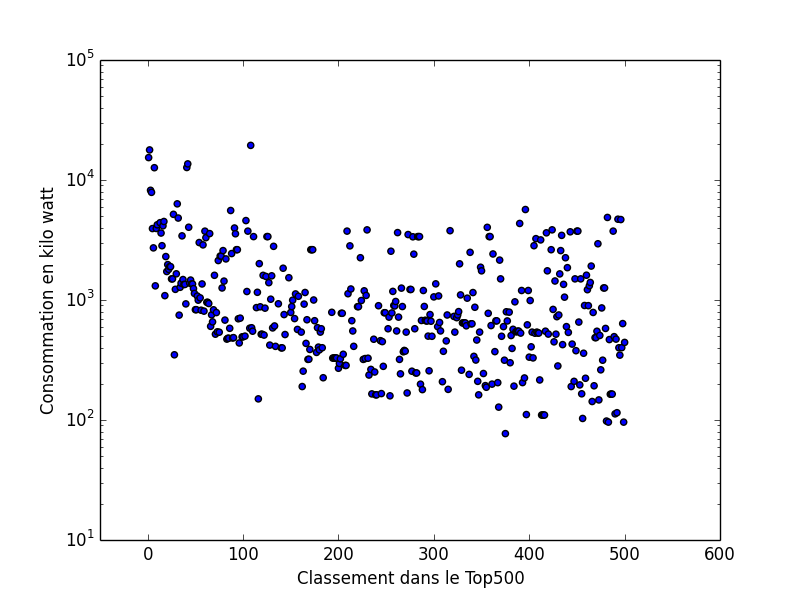
\includegraphics[width=10cm]{images/Chapitre1/pic_top500_power.png}
    \caption{\label{pic_top500_power} Consommation électrique des 500 supercalculateurs les plus puissants.}
\end{figure}



\subsubsection{Économique}
Le domaine du HPC est fortement influé par l'économie. En effet la construction de ces infrastructures coûte des millions d'euros d'investissement, et du fait que ces super-calculateurs sont des piliers stratégiques des entreprises, ces dernières sont très regardantes à leur coût. Cette forte pression de l'économie est une contrainte et il est difficile de proposer des sauts technologiques qui nécessitent de lourd investissement en amont sans connaître les retombés à l'avance. Comme vu dans la section consacré à l'énergie, nous devons repenser la façon dont nos codes sont conçus et exécutés. Par exemple en allant vers de nouvelles architectures comme les FPGA (Field Programmable Gate Array). Cette technologie permet de faire des périphériques très efficace en terme de consommation électriques. L'idée principale étant de laisser au programmeur le développement complet du circuit électronique pour qu'il corresponde parfaitement à son besoin. Mais la programmation de tels circuits est très complexe et demande des mois, souvent des années pour les codes complexes, pour être réalisée. Ainsi, malgré l'efficacité, prouvée, de cette technologie, les entreprises ne s'y lance pas à cause des coûts engendrés par les taille des équipes requises pour les programmer dans un temps raisonnable. On voit donc qu'il n'y a pas que les avancées et les nouvelles technologie qui sont importantes, il y a aussi leur facilité d'accès

\subsubsection{Technologiques}
Les différentes technologies connaissent elles aussi plusieurs contraintes. Une des principale à été exposé par Gordon Moore en 1965 qui a réalisé une conjecture qui est devenue la loi éponyme connus de tous. La loi de Moore prévoit que l'évolution du nombre de transistors sur une surface donnée va, grâce aux évolution technologique, être doublée tous les 2 ans à un prix constant. Sur la figure \ref{pic_Moore_prediction} on voit bien que cette évolution sur bel et bien la conjecture que le co-fondateur d'Intel a fait il y a plus de 50 ans.

\begin{figure}
    \center
    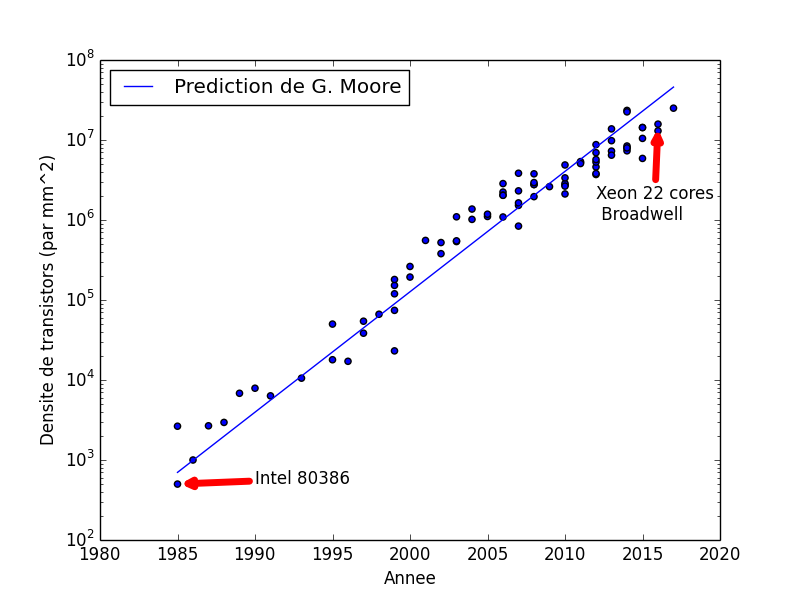
\includegraphics[width=10cm]{images/Chapitre1/Moore_prediction.png}
    \caption{\label{pic_Moore_prediction} La loi de Moore décrit l'évolution de la densité de transistors qui double tous les deux ans pour un prix constant (Données:  \url{https://en.wikipedia.org/wiki/Transistor_count}).}
\end{figure}


\textbf{TODO $Seminar_intro_v5.pdf$ slide 9 - expliquer moore par deux graphique: prix par mm2 et finesse de gravure}
Comme la puissance de calcul des processeurs est directement liée au nombre de transistors qu'ils contiennent, la puissance des puces à elle aussi suivi cette cadence. Alors pourquoi est ce devenu une contrainte ? Parce que pour doubler le nombre de transistors sans changer la surface gravée, il faut graver des transistors deux fois plus petits. Et si depuis 1965 on parvenait à le faire  au prix de nombreuses avancée techniques des appareils de gravure, nous atteignons aujourd'hui une limite physique, celle de la taille des atomes, voir figure \ref{pic_Moore_gravure}. En effet, aujourd'hui nous parvenons à graver des puces en autour de 10nm,  l'équivalent de quelques atomes. A cette taille les courants électriques ne sont plus stables et la course à la réduction des finesses de gravure est terminée. Alors qu'elle était un vecteur essentiel de l'évolution des performances, il va nous falloir trouver d'autres moyens pour arriver à atteindre l'exascale.

\textbf{TODO $Seminar_advanced technologies_v5.pdf$ slide 93 limite de Landauer}

\begin{figure}
    \center
    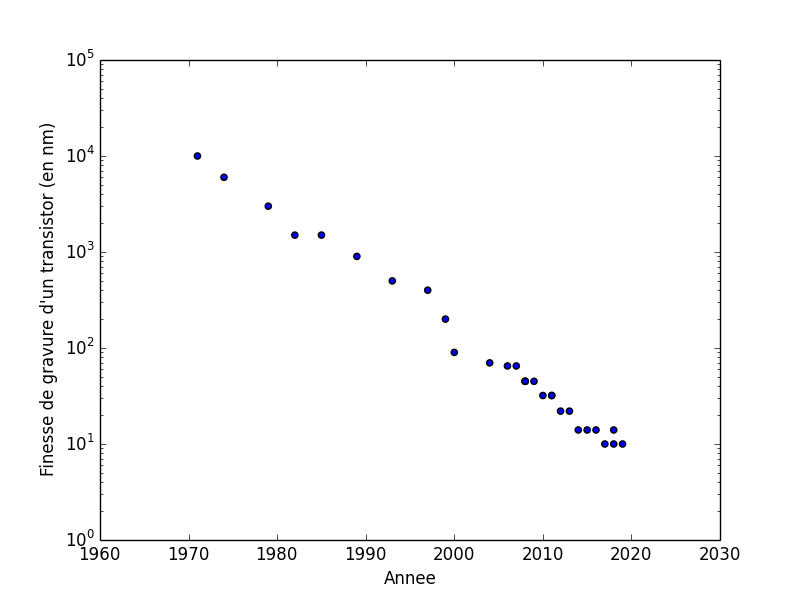
\includegraphics[width=10cm]{images/Chapitre1/Moore_gravure.png}
    \caption{\label{pic_Moore_gravure} La finesse des gravures à largement diminuée mais elle commence à toucher les limites de la physique \url{https://fr.wikipedia.org/wiki/Microprocesseur}).}
\end{figure}

La contrainte technique est très forte, d'autant plus avec l'apparition de nouvelles technologies plusieurs fois par ans. D'autant plus que souvent, ces nouveautés ne sont pas simplement des versions améliorées de précédents produits, ce sont souvent des technologies innovantes. Par exemple en c'est à partir de 2010 que l'on voit les premiers clusters contenant des cartes graphiques. Et il a fallut plusieurs années pour que cette technologie se fasse une place dans le monde du HPC notamment parce qu'elle nécessite une complète réécriture des codes. Il faut repenser la structure des algorithmes pour pouvoir tirer partie de tout le potentiel de ces cartes. Et il faut attendre 2013 pour voir une réelle percée de cette technologie (voir le graphique \ref{pic_GPU_repartition_TOP500}). Et il en est de même pour de nombreuses technologies innovantes, l'arrivée des mémoires non volatiles va demander aux utilisateurs de repenser une nouvelle fois leur algorithmes et seules des programmeurs expérimentés et avisés pourront le faire. L'exemple du FPGA est aussi un très bon exemple, sa complexité de programmation est un gros frein à son adoption. Et ces contraintes techniques se traduisent directement par un coût pour les entreprises. Car il faut engager des experts des différents domaines et investir de nombreuses heures pour faire les transformations adéquates.     


\begin{figure}
    \center
    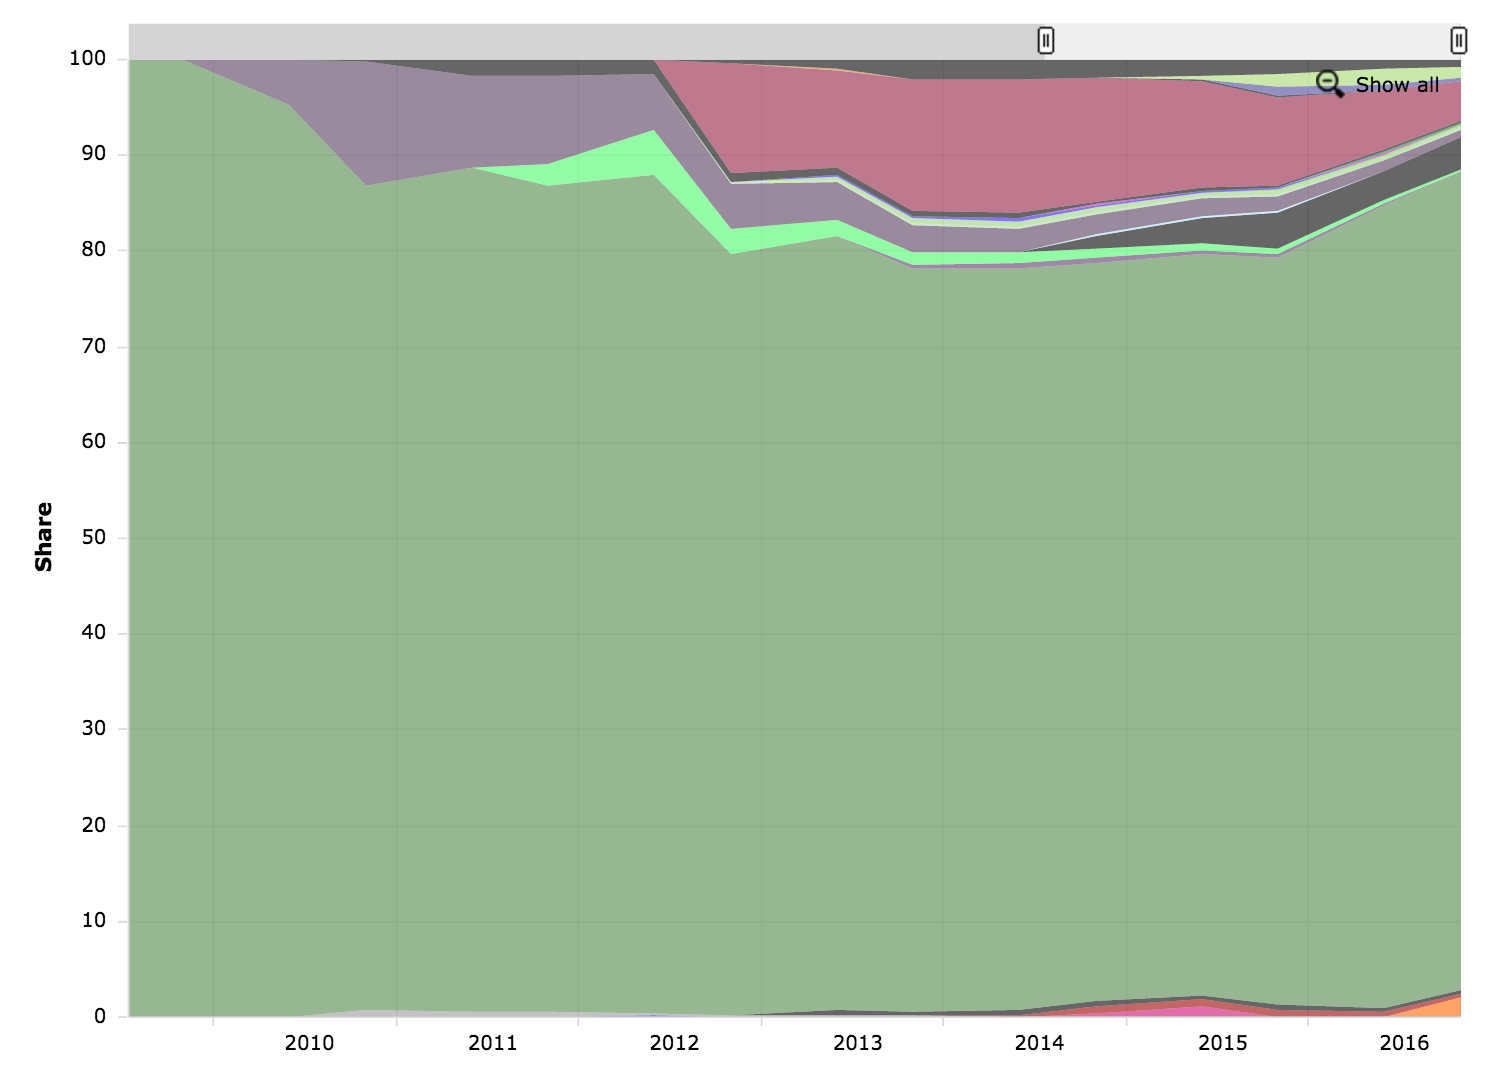
\includegraphics[width=10cm]{images/Chapitre1/pic_GPU_repartition_TOP500.png}
    \caption{\label{pic_GPU_repartition_TOP500} Partage de la performance totale du TOP500 entre les processeurs (couleur verte dominante) et les cartes graphiques (autres couleurs, représentants chaque modèles de cartes) \textit{source: \url{www.top500.org}}  }
\end{figure}

\subsubsection{Techniques et Connaissances}


Mes 3 ans d'expériences chez HPE et mon semestre de cours à Barcelone m'ont appris une chose: le domaine de l'analyse et des optimisations de performances est très difficile et nécessite de nombreuses connaissances et beaucoup d'expérience. La complexité des  architectures est telle qu'il est devenu impossible de prévoir avec précision leur comportement. Et ceci pour deux raisons: la première est le manque de connaissances fines de ces architectures et la deuxième est la faiblesse et la rareté des outils disponibles pour pour réaliser ce travail. En effet, pour contre balancer la complexité grandissante des architectures, il faut pouvoir utiliser des outils qui permettent de la comprendre. Or, la pauvreté des outils disponibles se fait ressentir et ceci pour une raison: personne n'en avait une réelle utilité jusqu'à maintenant. En réalité, il n'était pas nécessaire aux programmeurs de comprendre en détails toutes les finesses et toutes les particularités des architectures pour atteindre les performances voulues. Jusqu'à aujourd'hui il a suffit à l'industrie d'attendre les nouvelles versions des processeurs Intel (fameux modèle \textit{tic toc}) pour augmenter leur performances. Le travail d'optimisations ne valait alors pas le coup. C'est ainsi qu'aujourd'hui, alors que les contraintes se font plus pressantes que jamais, le domaine du HPC accuse le manques de développement d'outils et de formation de programmeur capable d'aller chercher ces performances.

De plus, les supercalculateurs se veulent de toujours plus hétérogènes en accueillant des accélérateurs diverses. Il faut donc calibrer les codes pour pouvoir être exécutés sur ces différentes architectures. Généralement, il faudra choisir un premier modèle de programmation dit à "mémoire distribuée". Il correspond à la partie du code qui s'occupe de partager le problème à résoudre entre les serveurs et qui s'occupe des communications. Le standard le plus utilisé celui de MPI (Message Passing Interface). Une fois le problème partagé, il faut coder le programme qui s'exécutera sur chaque serveurs, qui peuvent contenir plusieurs processeur. On utilise pour cela un deuxième paradigme de programmation, celui dit de "mémoire partagée". Enfin, ces serveurs peuvent aussi utilisé des accélérateurs (GPU, FPGA, DSP, etc.), il faudra donc écrire les programmes qui leur correspondent pour pouvoir les utiliser.
Les outils capables de nous aider dans ce travail nous manques et il est un objectif de cette thèse de fournir de tels outils. Mais il faut aussi user d'une méthodologie précise pour comprendre et optimiser ces codes. Fournir seulement un éventails d'outils ne sera pas suffisant si nous ne prodiguons pas les conseils que seule l'expérience peut apporter. Il est primordial de comprendre comment les codes sont exécutés sur nos système pour pouvoir espérer cibler de futures architectures comme \textit{The Machine}.







\subsection{Plateforme hétérogène}\label{sec:edl_hpc_hetero}
%%%%%%%%%%%%%%%%%%%%%%%%%%%%%%%%%%%%%%%%%%%%%%%%%%%
    
    On considère une plateforme hétérogène lorsque celle-ci possède au moins deux types d'unité de calculs. Les plateformes les plus répandues aujourd'hui possèdent un CPU x86 associé à un ou plusieurs GPU bien que d'autres architectures soient disponibles tels que les FPGA, DSP ou ASIC. Avec l'émergence d'applications adaptées à ces architectures et notamment les applications d'apprentissage par ordinateur, le nombre de supercalculateurs hétérogènes présent dans le Top500 n'a fait qu'augmenter ces 5 dernières années pour atteindre près d'un supercalculateur sur trois en 2019.
    
    \subsubsection{Avantages}
    %%%%%%%%%%%%%%%%%%%%%%%%%%%%%%
        Une grande partie des applications de calculs hautes performances bénéficie de l'utilisation des GPU dû à leur architecture ultra-parallèle. Les applications nécessitant des rendus visuels sont par exemple très adaptées à ce type d'accélérateur. 
    

    
    \subsubsection{Difficultés}
    %%%%%%%%%%%%%%%%%%%%%%%%%%%%%%
    
        Une difficulté pour utiliser de telles plateformes vient de la transformation du code qui doit être adaptée pour décomposer et répartir les données sur les différents noeuds de calculs pour réduire les transferts de données. De plus, les modèles de programmations utilisés sont généralement différents et d'autres langage tels que Cuda ou OpenCL doivent être utilisés. Ces transformations demandent un gros investissement des programmeurs. Une récente étude \cite{inproceedingsSCHC} conduite auprès de plusieurs industries montre que l'investissement nécessaire pour réaliser ces transformations est un frein majeur à l'adoption de ces architectures.
        
        La transformation du code est loin d'être évidente. Les langages, librairies et outils de programmation (debbuger, suivi de performance) sont moins avancés et robustes que ceux utilisés sur des architectures classiques. Les quatre entreprises interviewée constate le manque d'outils adaptés pour réaliser le travail du portage de code et de validation de performances. C'est une différence majeure entre l'industrie et le domaine de la recherche. Les applications industrielles sont plus complexes que celle utilisées comme démonstrateurs et il est souvent plus difficile d'atteindre les performances théoriques. Une entreprise témoignant dans l'étude \cite{inproceedingsSCHC} affirme que le manque d'expertise était le principale challenge pour le portage d'application. Ce constat est partagé par les autres entreprises présentées comme \textit{larges} et ayant les moyens d'embaucher de potentiels experts. 
        
        
        \textbf{TODO: }
        Actuellement, les GPUs sont les principaux accélérateurs utilisés dans les supersalculateurs (98\% des plateformes hétérogènes du Top500 en 2018). 
        
        
        On pourra cependant citer Google qui a développé son propre ASIC en 2015, le TPU, optimisé pour réaliser l'inférence de ses modèles d'apprentissage par machine learning. La phase d'inférence ne nécessite pas d'avoir autant de précision que la phase d'entraînement. Les ingénieurs ont donc développé le TPU utilisant des nombres flottants codés sur 8 bits. Cette réduction d'un facteur 8 permet de réduire la consommation électrique et la taille des circuits par un facteur 6 \cite{Jouppi2017}. La latence de réponse, importante pour la phase d'inférence, est entre 15 et 30 fois plus rapide que le GPU équivalent de l'époque (Nvidia K80)